\documentclass[a4paper,twocolumn]{article}

\usepackage[english]{babel}
\usepackage[utf8]{inputenc}
\usepackage{graphicx}
\usepackage{fullpage}

\usepackage{titlesec}

\titleformat*{\section}{\large\bfseries}
\titleformat*{\subsection}{\normalsize\bfseries}

\newcommand*\mean[1]{\overline{#1}}

\title{Convolutional Neural Fabrics $-$ summary}
\author{Matěj Nikl}

\begin{document}
\maketitle
Convolutional Neural Fabrics (CNFs) is a architecture for embedding an exponentially large number of CNN architectures (via massive parameter sharing). It is intended as a step aside from the conventional CNN model architecture selection problem $-$  it is not trying to solve it, instead it offers the opportunity for the fabrics to learn/select the most appropriate model (or even ensemble of models) within itself by standard back-propagation algorithm, leaving only the hyper-parameters of number of layers and channels up to us.
Other hyper-parameters, which are being ``set'' automatically by embedding in the fabrics are:
\begin{itemize}
    \item filter size per layer
    \item stride per layer
    \item number of pooling vs. convolutional layers
    \item type of pooling operator per layer
    \item size of the pooling regions
    \item ordering of pooling and convolutional layers
    \item channel connectivity pattern between layers
    \item type of activation (ReLU vs MaxOut)
\end{itemize}

% \section{Defining the Fabric}

\begin{figure}[!h]
    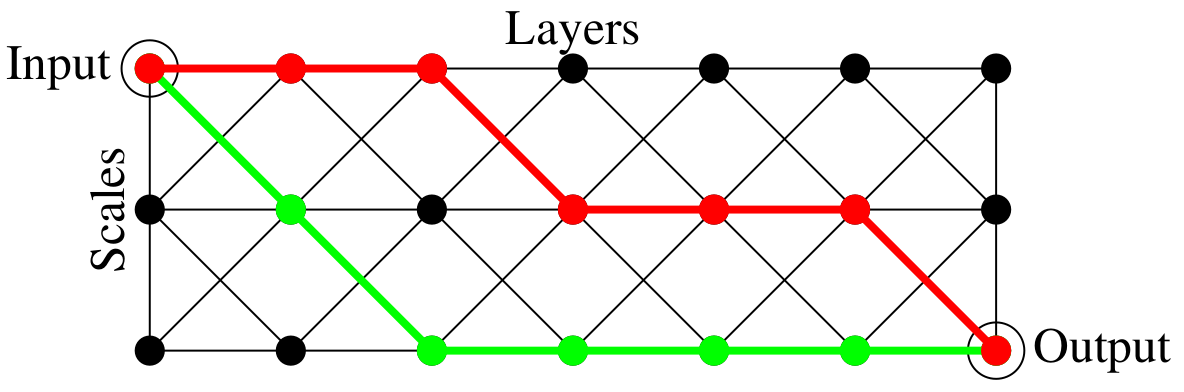
\includegraphics[width=\columnwidth]{fabrics1.png}
    \caption{Trellis embedding of two seven-layer CNNs. Trellis nodes receiving the input and producing output are encircled. All edges are oriented to the right, down in the first layer, and towards the ouput in the last layer. The channel dimension of the 3D trellis is omitted for clarity.}
\end{figure}

\section{Making sense of the Fabrics}
The Fabrics consist of a 3D trellis that connects response maps at different layers, scales, and channels with a sparse homogeneous local connectivity pattern.
Each node in the trellis represents a response map with the same number of dimensions as the input signal.

\subsection{The trellis structure}
It is spanned by three axes:
\begin{enumerate}
    \item a \textbf{layer} axis $-$ along which all edges advance, is analogous to the depth axis of a CNN
    \item a \textbf{scale} axis $-$ along which response maps of different resolutions are organized from fine to coarse
    \item a \textbf{channel} axis $-$ along which different response maps of the same scale and layer are organized
\end{enumerate}

Each node is connected to a 3 x 3 scale-channel neighborhood in the previous layer, i.e. channel $c$ at scale $s$ receives input from channels $\{c-1, c, c+1\}$ at scales $\{s-1, s, s+1\}$. Input from a finer scale is obtained via stride convolution, and input from a coarser scale by convolution, after upsampling by padding zeros around the activations at the coarser level.

\subsection{Embedded architectures}
\paragraph{Re-sampling operators}
Fine-to-coarse change of the resolution of response maps is done using stride-two convolutions. Larger strides can be obtained by following multiple such edges.

\textit{Average pooling} across small regions is alse strided convolution with uniform filter weights, thus available in the trellis. Average pooling over larger areas is also available.

\textit{Bi-linear interpolation} is commonly used in deconvolutional networks. Factor-two interpolation can be represented on coarse-to-fine edges by using a filter with $1$ in the center, $1/4$ on corners, and $1/2$ elsewhere. Larger powers of two can be obtained by repetition.

\begin{figure*}[t]
    \centering
    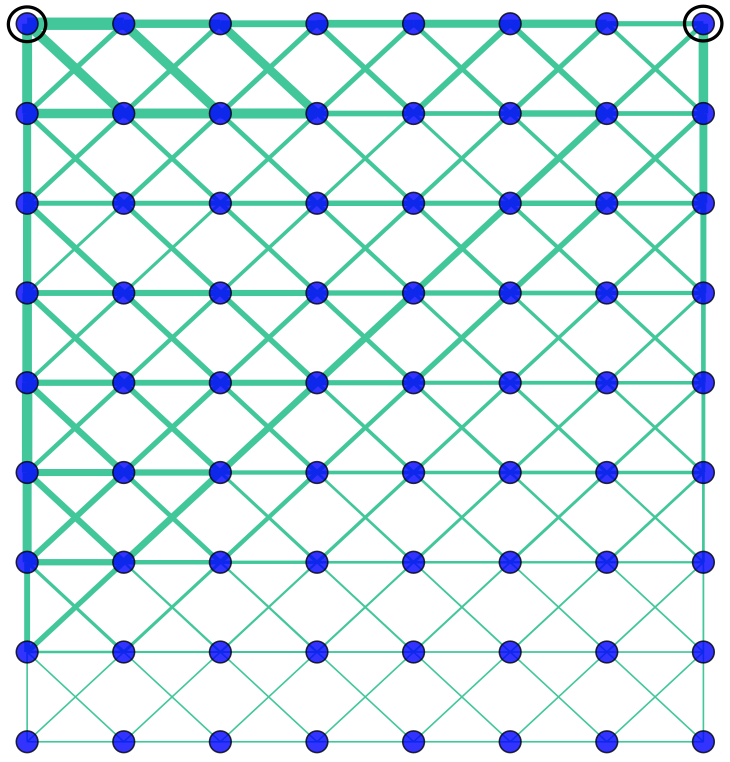
\includegraphics[width=0.375\textwidth]{fabrics2.png}
    \hskip 1cm 
    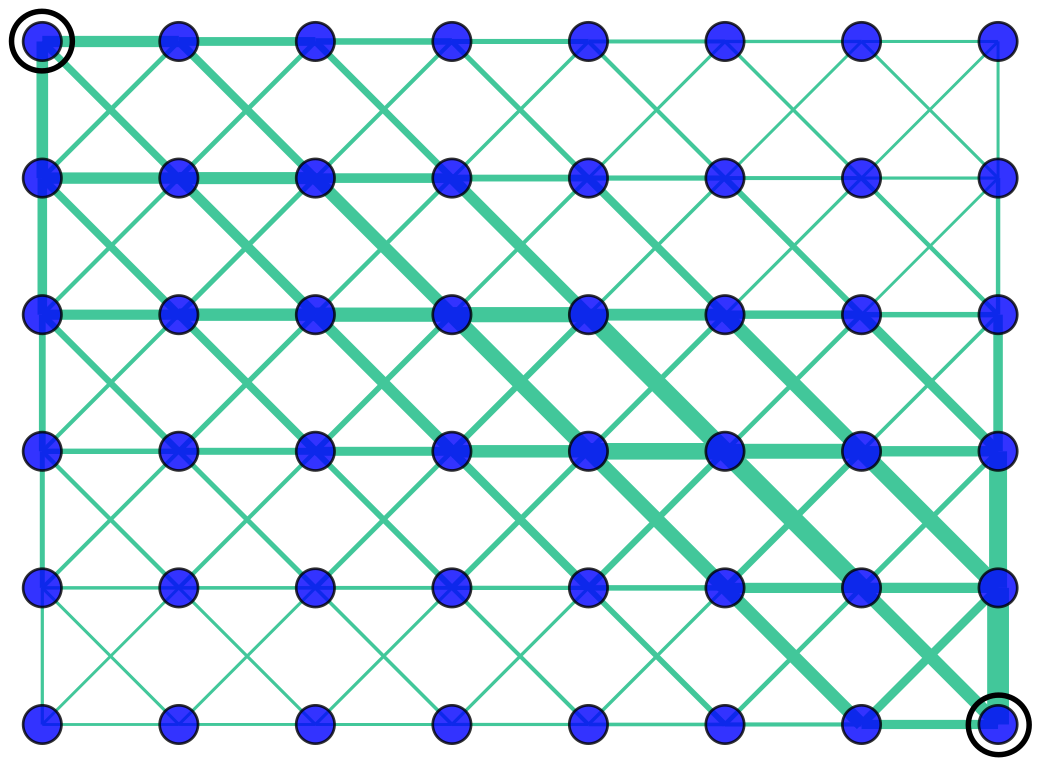
\includegraphics[width=0.5\textwidth]{fabrics3.png}
    \caption{Visualization of mean-squared filter weights (mean along weights and channels) in models learned for Part Labels (left) and MNIST (right). Layers are laid out horizontally, and scales vertically.}
\end{figure*}

\paragraph{Filter sizes}
A 5 x 5 filter can be implemented by computing nine intermediate channels to obtain a vectorized version of the 3 x 3 neighborhood at each pixel. A second 3 x 3 convolution can then aggregate values across the original 5 x 5 patch, and output the desired convolution. Repetition allows to implement every filter of any desired size.

\paragraph{Ordering convolution and re-sampling}
It is up to the back-propagation algorithm to choose the desired path(s) to use $-$ by setting all, exept one paths weights to zero, a particular sequence of convolutions and re-sampling operators is obtained.

\paragraph{Channel connectivity pattern}
This sparsely connected among che channel axis trellis suffices to emulate densely connected convolutional layers by copying channels, convolving them, and locally aggregating them.


\section{Principles of modularization}
The CNF architecture does not contain any standalone modules. The network itself can utilize some of its parts more, and by weight visualization it can be seen as modules being instationed, maybe even for certain purpopes, however they still make up a integral, inseparable part of the network.

\section{Principles of growing}
The CNF architecture does not allow for any more growing as a conventional (C)NN does. Its purpose is not in growing, but in dynamically utilizing its trellis structure, whilst hiding away multiple hyper-parameters.

\end{document}
